\chapter{推定に失敗したときの対策}\label{failure}

ここでは、最尤推定がうまくいかない場合の対処法についてまとめます。MNLモデルよりも高度なモデルを用いる場合、モデリングの誤りやバグが原因で推定が失敗することがあります。このような場合、どのようにデバッグを進めるべきかを図\ref{fig:estimation_failure}に示します。

\begin{figure}[ht]
    \centering
    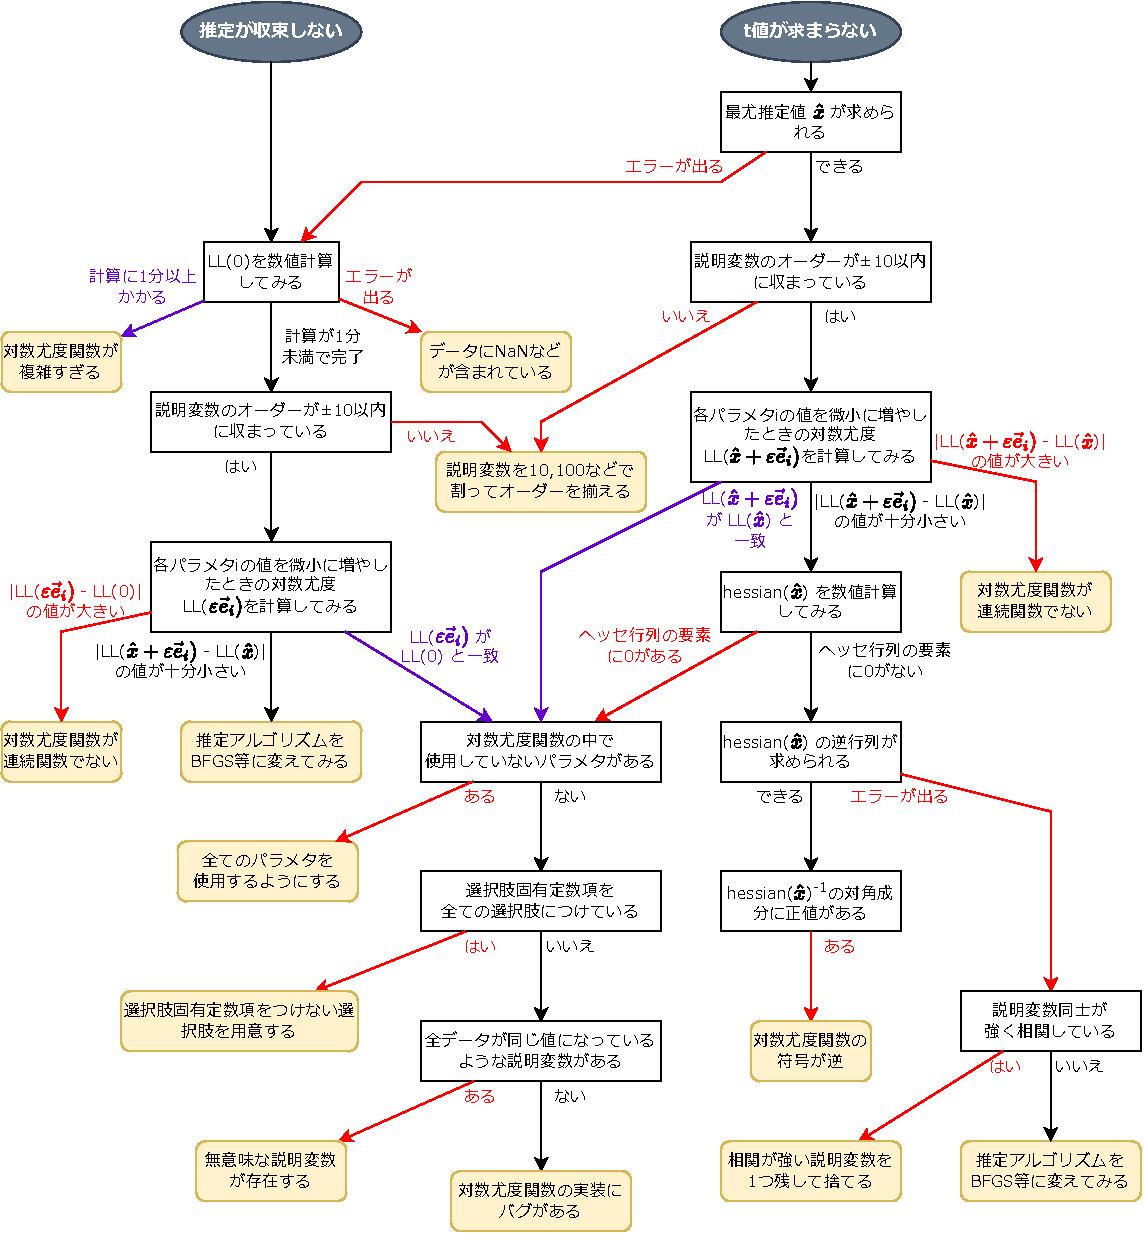
\includegraphics[width=0.95\hsize]{figure/estimation_failure.pdf}
    \caption{推定失敗時のデバッグフローチャート}
    \label{fig:estimation_failure}
\end{figure}
